% !TEX program = xelatex
% New URLs on AC, Fall 2026 — a broadside. One tabloid sheet of every network
% address the Aesthetic.Computer network learned to answer, 2026-08-16 → 09-15.
% Modelled on grants/culturehub-la-2026/acceptance/packet/program-broadside.tex.
\documentclass[10pt]{article}
\usepackage[paperwidth=12in,paperheight=18in,top=0.55in,bottom=0.5in,left=0.62in,right=0.62in]{geometry}
\usepackage{fontspec}
\usepackage{xcolor}
\usepackage{graphicx}
\usepackage{tabularx}
\usepackage{booktabs}
\usepackage{array}
\usepackage{ragged2e}
\usepackage{microtype}
\usepackage{tikz}
\usetikzlibrary{positioning,arrows.meta}
\usepackage{hyperref}
\hypersetup{colorlinks=true,urlcolor=acblue,linkcolor=acdark,pdftitle={New URLs on AC, Fall 2026}}

% Latin Modern by OTF filename: xelatex on macOS cannot resolve the family by
% name and silently falls back to nullfont (see papers/SCORE.md, cards lane).
\setmainfont{lmsans10-regular.otf}[
  BoldFont=lmsans10-bold.otf,
  ItalicFont=lmsans10-oblique.otf,
  BoldItalicFont=lmsans10-boldoblique.otf,
]
\setmonofont{lmmonolt10-regular.otf}[Scale=0.92,
  BoldFont=lmmonolt10-bold.otf,
  ItalicFont=lmmonolt10-oblique.otf,
]
% The YWFT display face: masthead only. Its punctuation is broken, so every
% dash, dot or slash inside a display string comes from the main font.
\newfontfamily\acbold{ywft-processing-bold}[Path=../../system/public/type/webfonts/,Extension=.ttf]
\newcommand{\dsep}{{\normalfont\;\textperiodcentered\;}}

\definecolor{acpink}{HTML}{B44887}
\definecolor{acpurple}{HTML}{7850B4}
\definecolor{acblue}{HTML}{1559A6}
\definecolor{acdark}{HTML}{312B38}
\definecolor{acgray}{HTML}{66636A}
\definecolor{acpale}{HTML}{F4F1F5}
\definecolor{acrule}{HTML}{DCD6DF}
\definecolor{acgreen}{HTML}{2D7650}
\definecolor{acorange}{HTML}{A85D24}
\newcommand{\acdot}{{\color{acpink}.}}
\newcommand{\ac}{Aesthetic{\acdot}Computer}

\pagestyle{empty}
\setlength{\parindent}{0pt}
\setlength{\parskip}{0pt}
\hyphenpenalty=10000\exhyphenpenalty=10000

% ── the vocabulary of the sheet ─────────────────────────────────────────
% \host{favicon}{name}{what it is}
\newcommand{\host}[3]{%
  \vspace{0.5em}%
  {\color{acdark}\rule{\linewidth}{1.6pt}}\par\vspace{0.3em}%
  {\raisebox{-0.22em}{\includegraphics[width=1.15em,height=1.15em]{figures/favicons/#1}}\ {\ttfamily\bfseries\fontsize{12.5pt}{14pt}\selectfont\color{acdark}#2}}\par\vspace{0.1em}
  {\fontsize{8pt}{9.6pt}\selectfont\color{acgray}\RaggedRight#3\par}\vspace{0.5em}}
% \addr{method}{path}{why}{date}{commit}{pill}
\newcommand{\addr}[6]{%
  \par\nointerlineskip{\color{acrule}\hrule height 0.5pt}\vspace{0.42em}%
  {\ttfamily\fontsize{8.8pt}{10.4pt}\selectfont{\bfseries\color{acpink}#1}\ {\bfseries\color{acdark}#2}}\par\vspace{0.12em}%
  {\fontsize{8.8pt}{10.6pt}\selectfont\color{acdark}\RaggedRight#3\par}\vspace{0.16em}%
  {\ttfamily\fontsize{7.2pt}{8.4pt}\selectfont\color{acgray}#4\ \ #5}\hfill#6\par\vspace{0.48em}}
\newcommand{\pill}[2]{{\fontsize{6.2pt}{7pt}\selectfont\colorbox{#1!12}{\textcolor{#1}{\bfseries\textls[60]{#2}}}}}
\newcommand{\live}{\pill{acgreen}{LIVE}}
\newcommand{\newhost}{\pill{acpink}{NEW HOST}}
\newcommand{\checkit}[1]{\pill{acorange}{#1}}
\newcommand{\hd}[1]{{\ttfamily\bfseries\fontsize{9pt}{10.3pt}\selectfont\color{acdark}#1}}
\newcommand{\lt}{\textless}\newcommand{\gt}{\textgreater}
% \changed{path}{what changed}
\newcommand{\changed}[2]{\par\nointerlineskip{\color{acrule}\hrule height 0.5pt}\vspace{0.3em}{\fontsize{8.3pt}{10pt}\selectfont\RaggedRight{\ttfamily\bfseries\color{acdark}#1}\ \ \color{acdark}#2\par}\vspace{0.3em}}

\begin{document}

% ═══════════════════════════════════════ masthead
{\ttfamily\fontsize{8.4pt}{10pt}\selectfont\color{acpink}\textls[80]{BROADSIDE\dsep AESTHETIC.COMPUTER\dsep WINDOW 2026-08-16 TO 2026-09-15}\par}
\vspace{0.3em}
{\acbold\fontsize{54pt}{52pt}\selectfont\color{acdark}New URLs on AC\ \ {\color{acpink}Fall 2026}\par}
\vspace{0.55em}
\begin{minipage}[t]{0.64\linewidth}\vspace{0pt}
{\fontsize{11.4pt}{14.2pt}\selectfont\color{acdark}\RaggedRight
Every address the \ac{} network learned to answer in the last thirty days, grouped by the host that answers it, in plain words. One sheet: what it is, what it is for, and when it opened.\par}
\vspace{0.45em}
{\fontsize{8.2pt}{10pt}\selectfont\color{acgray}\href{https://prompt.ac/@jeffrey}{\color{acblue}\textbf{@jeffrey}}\ \textperiodcentered\ \ac{}\ \textperiodcentered\ compiled 2026-09-15 from the git record\par}
\end{minipage}%
\hfill
\begin{minipage}[t]{0.32\linewidth}\vspace{0pt}
\renewcommand{\arraystretch}{0.9}
\begin{tabularx}{\linewidth}{@{}>{\raggedleft\arraybackslash}X>{\raggedleft\arraybackslash}X>{\raggedleft\arraybackslash}X@{}}
{\bfseries\fontsize{26pt}{26pt}\selectfont\color{acdark}19} & {\bfseries\fontsize{26pt}{26pt}\selectfont\color{acdark}5} & {\bfseries\fontsize{26pt}{26pt}\selectfont\color{acdark}2}\\
{\ttfamily\fontsize{6.6pt}{8pt}\selectfont\color{acgray}HTTP ROUTES} & {\ttfamily\fontsize{6.6pt}{8pt}\selectfont\color{acgray}NEW HOSTS} & {\ttfamily\fontsize{6.6pt}{8pt}\selectfont\color{acgray}MAIL DOORS}\\[0.5em]
{\bfseries\fontsize{26pt}{26pt}\selectfont\color{acdark}6} & {\bfseries\fontsize{26pt}{26pt}\selectfont\color{acdark}4} & {\bfseries\fontsize{26pt}{26pt}\selectfont\color{acpink}17}\\
{\ttfamily\fontsize{6.6pt}{8pt}\selectfont\color{acgray}SOCKET CHANNELS} & {\ttfamily\fontsize{6.6pt}{8pt}\selectfont\color{acgray}FLEET SERVICES} & {\ttfamily\fontsize{6.6pt}{8pt}\selectfont\color{acgray}DOORS CHANGED}\\
\end{tabularx}
\end{minipage}\par
\vspace{0.45em}
{\color{acdark}\rule{\linewidth}{3pt}}\par
\vspace{0.1em}

% ═══════════════════════════════════════ the map: three columns of hosts
\begin{minipage}[t]{0.315\linewidth}\vspace{0pt}

\host{aesthetic.computer.png}{aesthetic.computer/api/\ldots}{the main site's back room, served by lith, which redeploys itself on every push}
\addr{GET/POST}{/api/mail}{Your mailbox: inbox, sent, unread count and your addresses. Letters written with \texttt{tell} had been piling up here since April with no way to read them.}{2026-09-11}{a150032903}{\live}
\addr{GET}{/api/pruttivox?id=\ldots}{Speaks one of @prutti's chat messages in his consented voice clone, with per-word timing for karaoke. Renders are cached on Spaces.}{2026-09-08}{648e73a46e}{\live}
\addr{POST}{/api/prompt-log}{Records every prompt anyone submits, misses included. Admin can search it and pull counts.}{2026-09-03}{18f1271a5b}{\live}
\addr{GET/POST}{/api/mimechan}{An anonymous imageboard where the file's mimetype picks the board. Stored files are served under a sandbox policy.}{2026-09-02}{7f0af85c25}{\live}
\addr{POST}{/api/easel-inference}{Rents AI inference to a signed-in handle so an Easel install needs no vendor CLI. Metered by a daily per-handle budget.}{2026-09-12}{34d2f33d3d}{\live}
\addr{GET/POST}{/api/laklok-theme}{A census of which tema each laklok visitor wears. Both sister interfaces report on boot and on tap.}{2026-09-13}{b7037992a4}{\live}
\addr{GET}{/api/mediascholar-status}{Public progress of the Mediascholar paper worker. Also answers at papers.aesthetic.computer.}{2026-09-05}{467553fedb}{\live}

\host{aesthetic.computer.png}{inbound.aesthetic.computer:25}{SMTP, the mail door: the first way for the outside world to write to an AC handle. Only Google's relays may knock.}
\addr{SMTP}{\lt handle\gt @aesthetic.computer\newline \lt permahandle\gt @ \ \textperiodcentered\ \ amail+\lt permahandle\gt @}{Any handle is now an email address. The plus-tagged form is the return address on letters AC sends out, so replies find their way home.}{2026-09-13}{f6be8556c6 e8157fcb36}{\live\ \checkit{ROUTE SECRET UNSET}}
\addr{OUT}{smtp-relay.gmail.com}{Letters can leave the wall. They go out as ``@handle via aesthetic.computer'' and the domain now carries SPF and DKIM, so they land in inboxes.}{2026-09-13 / 09-14}{e8157fcb36 d3d9a8486c}{\live}

\vspace{0.3em}%
{\color{acdark}\rule{\linewidth}{1.6pt}}\par\vspace{0.18em}%
{\ttfamily\fontsize{7.6pt}{9pt}\selectfont\color{acpink}\textls[80]{HOW TO READ THIS}\par}\vspace{0.3em}
{\fontsize{7.9pt}{9.6pt}\selectfont\color{acgray}\RaggedRight
Every commit named here is on origin/main. lith redeploys itself on push, so the HTTP routes are presumed in production; the session server has watched for its own changes since 2026-09-11. {\color{acdark}\bfseries Live} was checked by hand on 2026-09-15 for the mail door, the TV host and the mailbox. {\color{acdark}\bfseries Route secret unset} means the mail door still logs that any Google tenant's route would be accepted. {\color{acdark}\bfseries Not on this sheet:} the feed worker (no changes), local-only MCP servers, the loopback credential proxy.\par
\vspace{0.3em}
Icons are the ones each host serves today. prompt.ac points its icon at a bucket that answers AccessDenied, so it wears the aesthetic.computer mark; so do the mail door, the session server and the fleet, which have no web icon. Source sweep in \texttt{endpoints-30d.md}. Set in YWFT Processing, Latin Modern Sans and Latin Modern Mono. \ac{}\par}

\end{minipage}%
\hfill{\color{acrule}\vrule width 1pt}\hfill
\begin{minipage}[t]{0.315\linewidth}\vspace{0pt}

\host{aesthetic.computer.png}{prompt.ac}{the short front door}
\addr{GET}{prompt.ac/easel.sh\newline /easel.tar.gz\ \textperiodcentered\ /easel.json}{One-line installer for Easel, the terminal coding tool. The tarball and manifest are packed on lith at deploy; the updater reads the manifest.}{2026-09-11}{6e02494c08 f9e68d9576}{\live}
\addr{GET}{prompt.ac/\textasciitilde\lt channel\gt}{The address a phone actually gets. Drops it straight into a live Aesthetic Code channel.}{2026-09-10}{cca4851c9e}{\live}
\addr{GET}{prompt.ac/\lt piece\gt}{Dotless paths now boot the HTML prompt in place instead of bouncing to aesthetic.computer. The Cloudflare redirect rule was switched off.}{2026-09-01}{a3b530ee4d}{\live}

\host{sotce.net.png}{sotce.net/sotce-net/\ldots}{the confessional}
\addr{GET}{/sw.js\ \textperiodcentered\ /manifest.json}{A push service worker and web-app manifest so pages, answers and chatter can ring readers' phones, iPhones included.}{2026-09-05}{91d70b972a d0cbaf7c4b}{\live}
\addr{POST}{/notification-choice}{Remembers each reader's bell choice and keeps a running count of who is opted in.}{2026-09-13}{2fed73e172}{\live}
\addr{GET}{/subscribers\ \textperiodcentered\ /active-subscribers}{Two numbers, split on purpose: the public subscriber count and the operational one that metrics reads.}{2026-09-13}{96bb08a349}{\live}
\addr{GET}{/comment (was /chat)\ \textperiodcentered\ www $\rightarrow$ sotce.net}{The chat room reads as a comment room now, and www folds into one canonical origin so Auth0, push and storage agree.}{2026-09-07}{bc12f6990c 8ab5f40c38}{\live}

\host{whistlegraph.org.png}{whistlegraph.org}{and its TV}
\addr{GET}{tv.whistlegraph.org}{The archive as broadcast: a zero-chrome fullscreen TV of whistlegraph performances. DNS checked today and answering.}{2026-08-16}{e861ac3e84}{\live}
\addr{GET}{/api/wg/verify?receipt=\&sig=}{A free check that a license receipt is genuine. The whole receipt is signed, so a code alone cannot forge one.}{2026-08-27}{c545a5444f}{\live}
\addr{GET}{/stars\ \textperiodcentered\ /comments\ \textperiodcentered\ /wild}{Three static rooms: the sky, what people said, and a field guide to sightings. Claimed by name so they are not mistaken for codes.}{09-01 / 09-03 / 09-05}{}{\live}

\end{minipage}%
\hfill{\color{acrule}\vrule width 1pt}\hfill
\begin{minipage}[t]{0.315\linewidth}\vspace{0pt}

\host{aesthetic.computer.png}{new hosts}{subdomains that did not exist in August}
\addr{}{
\includegraphics[width=0.95em,height=0.95em]{figures/favicons/aesthetic.computer.png}\ nft.aesthetic.computer + /data/*.json}{Cross-chain NFT portal with live media and holder snapshots served as plain JSON: catalog, RDP, a2p v2, ten whistlegraphs.}{2026-08-31}{d109bf8e1d}{\newhost}
\addr{}{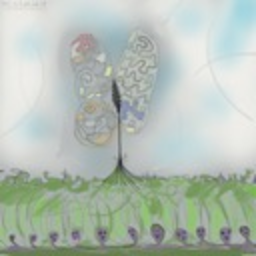
\includegraphics[width=0.95em,height=0.95em]{figures/favicons/rdp.aesthetic.computer.png}\ rdp.aesthetic.computer/json/1\ldots239}{Byte-faithful recovered metadata for all 239 RDP tokens, so the on-chain pointers resolve again.}{2026-08-31}{ff3ed1359a}{\newhost}
\addr{}{
\includegraphics[width=0.95em,height=0.95em]{figures/favicons/menuband.app.png}\ menuband.app $\rightarrow$ App Store}{The apex forwards straight to the Mac App Store page.}{2026-08-31}{b65327ef01}{\newhost}
\addr{}{
\includegraphics[width=0.95em,height=0.95em]{figures/favicons/aesthetic.computer.png}\ inbound.aesthetic.computer (https)}{Exists so certbot can mint the mail door's certificate. Says ``SMTP on :25'' and nothing else.}{2026-09-13}{318f1830c0 ae1933a8b7}{\newhost}

\host{aesthetic.computer.png}{wss://session-server\ldots}{live sockets; self-deploys every 60 s since 09-11}
\addr{WS}{/agent-presence?room=\lt handle\gt\newline \&role=agent\textbar surface}{Claude-in: an agent and a handle's screens can see each other, which lights the crab mark top-right.}{2026-09-03}{e72aa69a7b}{}
\addr{WS}{diagnostics:listen\ \textperiodcentered\ diagnostics:report}{A running piece can report on its own health, and only its author hears it.}{2026-09-11}{dd45600402}{}
\addr{GET}{/oskiewar-open-room\newline oskiewar:seat\ \textperiodcentered\ :input\ \textperiodcentered\ :net}{Strangers meet at the front door: the open versus room is public, and both seats now simulate the whole fight with rollback.}{09-03 / 09-05 / 09-09}{039b0cda33 c5121d2f97 c6a5729862}{}
\addr{WS}{chat:service-message}{YouTube live-chat viewers appear in the clock room as televised guests, authorised by a service secret rather than a person.}{2026-09-01}{c894adb754}{}

\host{aesthetic.computer.png}{fleet}{machines behind the site}
\addr{HTTP}{prox worker :5252\newline /job\ \textperiodcentered\ /poke\ \textperiodcentered\ /status/mediascholar}{Headless Linux job controller for the Mediascholar paper worker, LAN-bound. Its status is what the public status page proxies.}{2026-09-05}{ba66817f1d}{}
\addr{RTMP}{actv\ \textperiodcentered\ wgtv\ \textperiodcentered\ wgtv-playout\ \textperiodcentered\ tvchat}{Whistlegraph TV and laer-klokken TV, 24/7 to YouTube, with the chat bridge back into the clock room.}{2026-09-01}{2d867102e0 c894adb754}{}
\addr{AUTH0}{action: link-email-identity}{Runs in the Auth0 tenant: an emailed-code login merges into the account that already exists.}{2026-09-11}{d3d908bd77}{}

\end{minipage}\par

% ═══════════════════════════════════════ a letter's path (diagram)
\vspace{0.6em}
{\color{acdark}\rule{\linewidth}{1.6pt}}\par\vspace{0.35em}
{\ttfamily\fontsize{8pt}{9.5pt}\selectfont\color{acpink}\textls[80]{A LETTER'S PATH}\par}
\vspace{0.1em}
\begin{center}
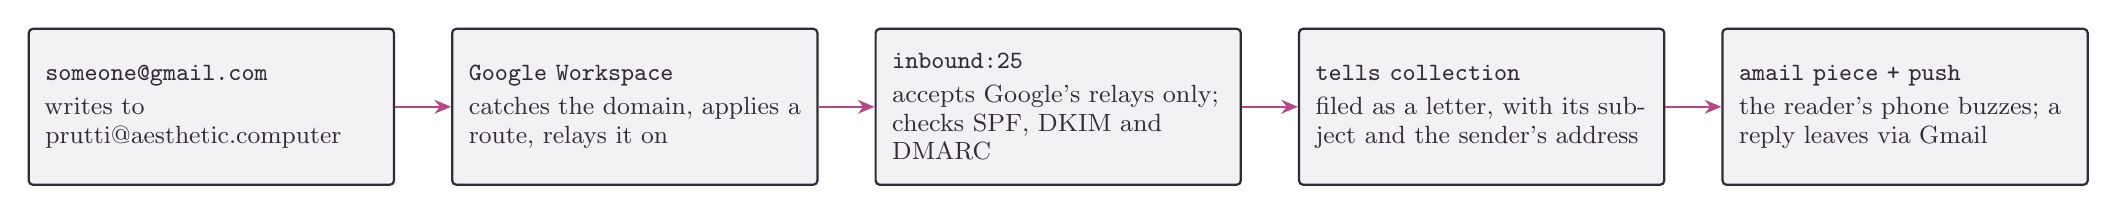
\begin{tikzpicture}[
  node distance=0.28in,
  box/.style={draw=acdark, line width=0.8pt, rounded corners=1.5pt, fill=acpale, text width=1.66in, minimum height=0.78in, align=left, inner sep=6pt, font=\fontsize{8.6pt}{10.3pt}\selectfont\color{acdark}},
  arr/.style={-{Stealth[length=6pt,width=5pt]}, line width=0.9pt, draw=acpink}
]
\node[box] (a) {\hd{someone@gmail.com}\\[2pt]writes to prutti@aesthetic.computer};
\node[box, right=of a] (b) {\hd{Google Workspace}\\[2pt]catches the domain, applies a route, relays it on};
\node[box, right=of b] (c) {\hd{inbound:25}\\[2pt]accepts Google's relays only; checks SPF, DKIM and DMARC};
\node[box, right=of c] (d) {\hd{tells collection}\\[2pt]filed as a letter, with its subject and the sender's address};
\node[box, right=of d] (e) {\hd{amail piece + push}\\[2pt]the reader's phone buzzes; a reply leaves via Gmail};
\draw[arr] (a) -- (b); \draw[arr] (b) -- (c); \draw[arr] (c) -- (d); \draw[arr] (d) -- (e);
\end{tikzpicture}
\end{center}
\vspace{0.3em}

% ═══════════════════════════════════════ footer: changed doors + colophon
{\color{acdark}\rule{\linewidth}{3pt}}\par\vspace{0.45em}
{\ttfamily\fontsize{8pt}{9.5pt}\selectfont\color{acpink}\textls[80]{DOORS THAT WERE ALREADY OPEN BUT CHANGED SHAPE}\par}\vspace{0.35em}
\begin{minipage}[t]{0.315\linewidth}\vspace{0pt}
\changed{/api/ask}{daily token budget per handle; anonymous callers get the cheap model only.}
\changed{/run}{a handle/slug channel needs that handle's token. Ownership is the token, not the secret name.}
\changed{/api/tell}{now lands in the recipient's mail; letter text kept out of push bodies and logs.}
\changed{/api/say}{any signed-in handle may send text; the prutti voice is producer-gated.}
\end{minipage}\hfill
\begin{minipage}[t]{0.315\linewidth}\vspace{0pt}
\changed{/api/version}{long-poll held 45 s instead of 4 s. It was 57\% of daily requests.}
\changed{/api/oskiewar-replays}{anonymous seat may upload; rooms named on round summaries.}
\changed{/api/register-push-token}{sotce tenant and topics for pages and chat.}
\changed{/api/chat-messages}{rows carry who relayed them and a YouTube walk-back link.}
\end{minipage}\hfill
\begin{minipage}[t]{0.315\linewidth}\vspace{0pt}
\changed{/api/piece-hit}{bots counted but flagged; a stray socket upgrade gets a 426 pointing at the session server.}
\changed{/api/nom-scores}{numrank game added; score-only runs.}
\changed{/api/wg/*}{facilitator signs every call with a fresh Ed25519 JWT.}
\changed{caddy cache}{worker bundle immutable; bios and disk no-cache; oskiewar modules precompressed.}
\end{minipage}\par
\end{document}
